\chapter{Introduction}

Ce chapitre introductif a pour but d'illustrer les objets qui seront étudiés plus rigoureusement dans la suite de ce cours. L'objectif est donc de donner des représentations er de se forger un état d'esprit pour comprendre les notions de manière plus abstraites.    

\section{Notations et rappels de base}

Sauf précisions particulières les symboles suivants désignent :
\begin{itemize}
	\item $\N = \left\{ 0,1,2,3,\cdots \right\}$ est l'ensemble des entiers naturels
	\item $n$ est un entier naturel strictement positif
	\item $\R$ est l'ensemble de nombres réels
	\item $\R\times \cdots \times \R^n$ est l'ensemble des $n$-uplet de nombres réels. 
	\item si $\x$ est un élément de $\R^n$ : Pour $n=2$ on note $\x= (x_1,x_2)=\begin{psmallmatrix}x_1\\x_2\end{psmallmatrix}$ ou $\x=(x,y) = \begin{psmallmatrix}x\\y\end{psmallmatrix}$ selon l'humeur. De même pour $n=3$, on note indifféremment $\x=(x_1,x_2,x_3) = \begin{psmallmatrix}x_1\\x_2\\x_3\end{psmallmatrix}$ ou $\x=(x,y,z)=\begin{psmallmatrix}x\\y\\z\end{psmallmatrix}$.
\end{itemize}

\section{Rappel de géométrie du plan et de l'espace}

Dans cette partie, on considère les vecteurs du plan ou de l'espace. Ce chapitre est une introduction informelle à la géométrie vectorielle élémentaire et a pour but de vous familiariser avec des notions et techniques utilisées dans la suite du cours. Certaines définitions seront vues plus rigoureusement dans la suite.

%On fixe une origine $O$ de l'espace, il revient donc au même de parler de $\R^2$ ou $\R^3$.

\subsection{Points et vecteurs}

On modélise le plan et l'espace par des espaces affines de dimension 2 et 3 respectivement.

Pour l'espace à 3 dimension $\mathcal E$ on considère l'ensemble $\R^3$ des triplet de réels. On peut en effet décrire un point $M$ de l'espace par un triplet $(x,y,z)\in\R^3$ de réels. D'un autre coté, on peut voir $\R^3$ comme un espace vectoriel noté $E$. Un vecteur $u\in E$ modélise alors un ``déplacement'' entre 2 points $A$ et $B$ de $\Ee$. Si $A = (a_1,a_2,a_3)$ et $B=(b_1,b_2,b_3)$ on définit le vecteur $u = \overrightarrow{AB}$ comme étant le triplet de réels $u = (b_1-a_1,b_2-a_2,b_3-a_3)$. %On note généralement $u= \overrightarrow{AB}$.
%Les règles de calculs usuelles 
En résumé, les éléments de $\Ee$ sont considérés comme des points (noté en majuscule) sur lesquels opèrent des vecteurs (en minuscule).

La relation entre couple de points (on parle de bipoints) et vecteur est précisé dans la définition suivante :%On peut axiomatiser la construction des espaces affines avec la définition suivante :
\begin{definition}
	Soit $E$ un \rev. Un espace affine dirigé par $E$ est un ensemble $\mathcal E$ non vide, muni d'une application $\varphi : \mathcal E \times \mathcal E \to E$ vérifiant les axiomes suivants :
	\begin{itemize}
		\item pour tout $A,B,C\in \mathcal E$ on a $\varphi(A,C) = \varphi(A,B) +  \varphi(B,C)$ (\emph{relation de Chasles}),
		\item pour tout $A \in \mathcal E$ et pour tout $x\in E$, il existe un unique $B \in \mathcal E$ tel que $x = \varphi(A,B)$ (\ie l'application $\varphi_A:M\mapsto\varphi(A,M)$ est une bijection de $\mathcal E$ dans $E$).
	\end{itemize}
\end{definition}
Dans le cas du plan ou de l'espace, un couple de points $(A,B)$ est un bipoint auquel on associe le vecteur $\varphi(A,B)$ qui est noté $\overrightarrow{AB}$.

\subsection{Repère de l'espace} 

\begin{definition}[(Repère cartésien)]
Un repère cartésien de l'espace $\Ee$ est la donnée d'un point $\Omega$ (l'origine du repère) et de trois vecteurs $(e_1,e_2,e_n)$ formant une base (\ie une famille libre maximale) de l'espace $E$.
\end{definition}

\begin{definition}[(coordonnées cartésiennes)]
	Si $M$ est un point de $\Ee$ alors le vecteur $\overrightarrow{\Omega M}$ se décompose de façon unique sur les vecteurs de base :
	\[
		\overrightarrow{\Omega M} = x_1 e_1 + x_2 e_2 + x_3 e_3 
	\]
	Le triplet $\begin{psmallmatrix}x_1 \\ x_2 \\ x_3\end{psmallmatrix}_{\mathcal R}$ (ou plus simplement $(x_1,x_2,x_3)$ si il n'y a pas d'ambiguïtés) contient les coordonnées cartésiennes du point $M$ dans le repère $\mathcal R$.
\end{definition}

\begin{remark}
	Une fois le repère fixé, il revient au même de considérer $\Ee$ (plan ou espace) ou des espaces vectoriel $E=\R^3$. %On peut ainsi utiliser tous les résultats d'algèbre linéaire : coordonnées d'un veet la formule de changement de base.
\end{remark}

Soient deux repères cartésiens $\mathcal R =(\Omega,e_1,e_2,e_3) $ et $\mathcal R' =(\Omega',e_1',e_2',e_3') $ et un point $M$. On note :
\begin{itemize}
	\item $\begin{psmallmatrix}x\\ y \\z \end{psmallmatrix}_{\mathcal R}$ les coordonnées de $M$ dans $\mathcal R$ et $\begin{psmallmatrix}x'\\y'\\z' \end{psmallmatrix}_{\mathcal R'}$ les coordonnées de $M$ dans $\mathcal R'$
	\item $\begin{psmallmatrix}\alpha\\\beta\\\gamma \end{psmallmatrix}_{\mathcal R}$ les coordonnées de $\Omega'$ dans la $\mathcal R$.
	\item $\begin{psmallmatrix} a_{1,i}\\a_{2,i}\\a_{3,i} \end{psmallmatrix}_{\mathcal R}$ les coordonnées de $e_i'$ ($i=1,2,3$) dans $\mathcal R$.
\end{itemize}
%Pour passer d'un reprère à l'autre on a la formule suivante : 
Alors les coordonnées du point $M$ dans le repère $\mathcal R$ s'expriment en fonction des coordonnées de $M$ dans le repère $\mathcal R$ :
\[
	\begin{cases}
		x = \alpha +a_{1,1}x'+ a_{1,2}y' +a_{1,3} z'\\
		y = \beta  +a_{2,1}x'+ a_{2,2}y' +a_{2,3} z'\\
		z = \gamma +a_{3,1}x'+ a_{3,2}y' +a_{3,3} z'
	\end{cases}
\]

%\begin{remarque}
	%Si on condidère 2 repères orthonormés d
%\end{remarque}

\begin{definition}
	[(Droite vectorielle, droite affine)]
	\begin{enumerate}
		\item Dans $E$ : la \emph{droite vectorielle} engendrée par un vecteur $u$ non-nul est l'ensemble des vecteurs colinéaire à $u$ :
			\[
				\vect(u) = \left\{ v\in E, \exists \lambda \in \R, v = \lambda u \right\}
			\]

		\item	Dans $\mathcal E$ : la \emph{droite affine} $\mathcal D$ passant par un point $A$ et dirigée par un vecteur non-nul $u$ est l'ensemble des points $\mathcal D = \left\{ A + \lambda u, \lambda \in \R \right\}$. On note $\mathcal D = A + \vect (u)$ et on dit que $\vect(u)$ est la direction de $\mathcal D$.
	\end{enumerate}
\end{definition}

\subsection{Orientation de l'espace}

Un repère $\left\{ 0,e_1,e_2,e_3 \right\}$ de l'espace à deux orientations possibles. Il faut donc faire un choix et choisir une convention. On se contente ici de décrire le choix usuel à l'aide de l'une des règles classique (``règle des 3 doigts de la main droite'', règle du ``bonhomme d'ampère'', règle du ``tire bouchon''\ldots). On dit qu'un repère est \emph{direct} si le pouce, l'index et le majeur de la main droite peuvent être placés (direction et sens) suivant les vecteurs $(e_1,e_2,e_3)$.
%On privilégiera bien sûr la représentation directe des axes $(Ox,Oy,Oz)$ :
\begin{center}
	\begin{tabular}{cc}
		% version with pst-figure3d
%\psset{viewpoint=50 20 30 rtp2xyz,Decran=50}
%\begin{pspicture}[solidmemory](-4,-4)(6,5)
%%\psset{unit=0.5}

%\psSolid[object=plan,action=draw,definition=equation,args={[0 0 1 0]}, base=-4 4 -4 4,fillcolor=black!15,fillstyle=solid,name=P0]
%\psProjection[object=texte,fontsize=100,linecolor=red,text=slice,phi=90,plan=P0]

%%\psSolid[object=cube,a=8,action=draw,name=A,linecolor=red]

%%\psSolid[object=plan,action=none,definition=solidface,args=A 4,name=P1]
%%\psProjection[object=texte,fontsize=50,text=lateral,phi=-90,plan=P1](-5,0)

%\psSolid[object=plan,action=draw,definition=equation,args={[0 1 0 0]},opacity=.2, base=-4 4 -4 4,fillcolor=black!15,name=P2]
%%\psProjection[object=texte,fontsize=50,text=axial,phi=90,plan=P2](0,7)
%%\psSolid[object=plan,action=none,definition=equation,args={[1 0 0 0]},name=P3]
%%\psProjection[object=texte,action=draw,fontsize=50,text=temporal,phi=90,plan=P3](4,8)
%\axesIIID(0,0,0)(4,4,4)
%\end{pspicture}

%\psset{unit=0.45}
%\psset{viewpoint=50 40 30 rtp2xyz,Decran=50}
%\psset{lightsrc=viewpoint}
%\begin{pspicture}(-7,-8)(7,8)
%\psSurface[ngrid=.25 .25](-4,-4)(4,4){((y^2)-(x^2))/4 }
%\end{pspicture}

%\psset{viewpoint=30 40 20 rtp2xyz,Decran=30}
  %\begin{pspicture}(-3.5,-3.5)(3.5,3.5)
%%  \axesIIID(2,2,2)(4,4,4)
   %\psSolid[object=cube,a=4,fillcolor=blue,opacity=0.2,action=draw*]%
   %\psSolid[object=sphere,r=1.5,linewidth=0.1pt,ngrid=20 20,fillcolor=red,opacity=0.2,action=draw*]%
   %\psSolid[object=vecteur,args=0 -2 0](2,2,-2)
   %\psSolid[object=vecteur,args=-2 0 0](2,2,-2)
   %\psSolid[object=vecteur,args=0 0 2](2,2,-2)
   %\psPoint(2,2,0.2){Z}\rput(Z){z}\psPoint(2,-0.2,-2){X}\rput(X){x}\psPoint(-0.2,2,-2){Y}\rput(Y){y}
   %\psPoint(2,-1.6,-2){a1}\psPoint(2,-1.6,2){a2}\pcline{<->}(a1)(a2)\ncput*{d}
   %\psPoint(2,-1.6,2){a1}\psPoint(-2,-1.6,2){a2}\pcline{<->}(a1)(a2)\ncput*{d}
   %\psPoint(-1.6,2,-2){a1}\psPoint(-1.6,2,2){a2}\pcline{<->}(a1)(a2)\ncput*{d}
   %\psPoint(0,0,0){a1}\psPoint(1,-1,0){a2}\pcline{->}(a1)(a2)\ncput*{r}
  %\end{pspicture}

%\begin{tikzpicture}
%\def\zlength{-0.5cm}
%\foreach \zangle [count=\i from 0] in {10,30,...,80}{
%\begin{scope}[shift={({mod(\i,2)*4cm},{-floor(\i/2)*4cm})}, 
    %x=(0:1cm), y=(90:1cm),z=(\zangle:\zlength)]
%%\def\zangle{80}
    %\def\sliceZ{0}
    %\def\side{2}
    %% draw plane
    %\filldraw[color=gray!40] (0,0,0) -- (0,0,\side) -- (\side,0,\side) -- (\side,0,0) -- cycle;
    %\filldraw[color=gray!40] (0,0,0) -- (0,\side,0) -- (\side,\side,0) -- (\side,0,0) -- cycle;
    %\filldraw[color=gray!40] (0,0,0) -- (0,0,\side) -- (,0\side,\side) -- (0,\side,0) -- cycle;
     %%\draw[dashed] (0,\sliceZ,0) -- (0,\sliceZ,\side) -- (\side,\sliceZ,\side) -- (\side,\sliceZ,0) -- cycle;
    %% draw axes
    %\draw[->] (0,0,0) -- (\side+.3,0,0) node[right] {$x$};
    %\draw[->] (0,0,0) -- (0,\side+.3,0) node[below] {$y$};
    %\draw[->] (0,0,0) -- (0,0,\side+.3) node[below] {$z$};
    %\node[cm={1,0,cos(\zangle),sin(\zangle),(0,0)}] at (1,1,0){plan $x-y$};
    %\node[cm={1,0,cos(\zangle),sin(\zangle),(0,0)}] at (1,0,1){plan $x-z$};
    %\node[cm={1,0,cos(\zangle),sin(\zangle),(0,0)}] at (0,1,1){plan $x-z$};
%\end{scope}
%}
%\end{tikzpicture}
\begin{tikzpicture}
    [%x={(-0.5cm,-0.5cm)},
%	    y={(1cm,0cm)},
%	    z={(0cm,1cm)}, 
    scale=1,
    fill opacity=1,%0.80,
    very thin,
    every node/.append style={transform shape}]
\newcommand\drawface{\draw[fill=gray!100] (-.2,-.2) rectangle (2,2)}

\def\ctr{1}
\def\side{2}
\def\sideT{.4}
\filldraw[color=green!40] (-\sideT,-\sideT,0) -- (-\sideT,\side,0) -- (\side,\side,0) -- (\side,-\sideT,0) -- cycle;
\filldraw[color=blue!40] (-\sideT,0,-\sideT) -- (-\sideT,0,\side) -- (\side,0,\side) -- (\side,0,-\sideT) -- cycle;
\filldraw[color=gray!40] (0,-\sideT,-\sideT) -- (0,-\sideT,\side) -- (0,\side,\side) -- (0,\side,-\sideT) -- cycle;

\def\sideT{0}
\filldraw[color=green!40] (-\sideT,-\sideT,0) -- (-\sideT,\side,0) -- (\side,\side,0) -- (\side,-\sideT,0) -- cycle;
\filldraw[color=blue!40] (-\sideT,0,-\sideT) -- (-\sideT,0,\side) -- (\side,0,\side) -- (\side,0,-\sideT) -- cycle;
\filldraw[color=gray!40] (0,-\sideT,-\sideT) -- (0,-\sideT,\side) -- (0,\side,\side) -- (0,\side,-\sideT) -- cycle;
	% face #3
	\begin{scope}[canvas is zx plane at y=0]
	   %\drawface;
		\draw[thick,->] (1.5,1) arc (0:90:.5cm) node[above right,midway]{$+$};
	   \node[rotate=90] at (\ctr/2,\ctr) {plan $xy$};
	\end{scope}
	% face #2
	\begin{scope}[canvas is yx plane at z=0]
	   %\drawface;
		\draw[thick,<-] (1.5,1) arc (0:90:.5cm) node[above right,midway]{$+$};
	   \node[yscale=-1,rotate=-90] at (\ctr/2,\ctr) {plan $yz$};
	\end{scope} 

       % face #1
	\begin{scope}[canvas is yz plane at x=0]
	    %\drawface;
		\draw[thick,->] (1.5,1) arc (0:90:.5cm) node[above right,midway]{$+$};
	    \node[rotate=-90] at (\ctr/2,\ctr) {plan $xz$};
	\end{scope}



	\draw[thick,->] (0,0,0) -- (\side+.3,0,0) node[right,text width=2.1cm, align=center] {$y$ (index)};
	\draw[thick,->] (0,0,0) -- (0,\side+.3,0) node[above,text width=2.4cm, align=center]{$z$ (majeur)} ;
	\draw[thick,->] (0,0,0) -- (0,0,\side+.3) node[below left,text width=2cm, align=center] {$x$ (pouce)};
\end{tikzpicture}
 & 
		%\usetikzlibrary{3d}
\begin{tikzpicture}
	[%x={(-0.5cm,-0.5cm)},
%	    y={(1cm,0cm)},
%	    z={(0cm,1cm)}, 
		scale=1,
		fill opacity=1,%0.80,
		very thin,
	every node/.append style={transform shape}]

\def\ctr{1}
\def\side{2}
\def\sideT{.4}
\filldraw[color=blue!40] (-\sideT,-\sideT,0) -- (-\sideT,\side,0) -- (\side,\side,0) -- (\side,-\sideT,0) -- cycle;
\filldraw[color=gray!40] (-\sideT,0,-\sideT) -- (-\sideT,0,\side) -- (\side,0,\side) -- (\side,0,-\sideT) -- cycle;
\filldraw[color=green!40] (0,-\sideT,-\sideT) -- (0,-\sideT,\side) -- (0,\side,\side) -- (0,\side,-\sideT) -- cycle;

\def\sideT{0}
\filldraw[color=blue!40] (-\sideT,-\sideT,0) -- (-\sideT,\side,0) -- (\side,\side,0) -- (\side,-\sideT,0) -- cycle;
\filldraw[color=gray!40] (-\sideT,0,-\sideT) -- (-\sideT,0,\side) -- (\side,0,\side) -- (\side,0,-\sideT) -- cycle;
	\filldraw[color=green!40] (0,-\sideT,-\sideT) -- (0,-\sideT,\side) -- (0,\side,\side) -- (0,\side,-\sideT) -- cycle;

%	% face #3
	\begin{scope}[canvas is zx plane at y=0]
		\draw[thick,->] (1.5,1) arc (0:90:.5cm) node[above right,midway]{$+$};
		\node[rotate=90] at (\ctr/2,\ctr) {plan $xz$};
	\end{scope}
%	% face #2
	\begin{scope}[canvas is yx plane at z=0]
		\draw[thick,<-] (1.5,1) arc (0:90:.5cm) node[above right,midway]{$+$};
		\node[yscale=-1,rotate=-90] at (\ctr/2,\ctr) {plan $xy$};
	\end{scope} 
%
%      % face #1
	\begin{scope}[canvas is yz plane at x=0]
		\draw[thick,->] (1.5,1) arc (0:90:.5cm) node[above right,midway]{$+$};
		\node[rotate=-90] at (\ctr/2,\ctr) {plan $yz$};
	\end{scope}

	\draw[thick,->] (0,0,0) -- (\side+.3,0,0) node[right,text width=2cm, align=center] {$x$ (pouce)};
	\draw[thick,->] (0,0,0) -- (0,\side+.3,0) node[above,text width=2.1cm, align=center] {$y$ (index)};
	\draw[thick,->] (0,0,0) -- (0,0,\side+.3) node[below left,text width=2.4cm, align=center] {$z$ (majeur)};

\end{tikzpicture}

	\end{tabular}
\end{center}
Une permutation circulaire de trois vecteurs ne modifie pas son orientation et les deux repères ci-dessus sont directs. Si on change l'orientation d'un des vecteurs, on change l'orientation du repère (orientation \emph{indirect}). Dans la suite de ce cours nous considèrerons toujours des repères directs.

\subsection{Produit scalaire}

\subsubsection{définition}
On se place dans l'espace vectoriel $E = \R^3$ muni de la base canonique $i = (1,0,0)$, $j=(0,1,0)$ et $k=(0,0,1)$. 

\begin{definition}
	Soit $u =(u_1,u_2,u_3)$ et $v=(v_1,v_2,v_3)$ deux vecteurs de $\R^3$. Le produit scalaire est \[
		\prs{u,v} = u_1v_1 + u_2v_2 + u_3v_3.
	\]
et on définit la \emph{norme} d'un vecteur $u=(x,y,z)$ par
\[
	\norm{u}  = \sqrt{x^2+y^2+z^2}.
\]
\end{definition}

On a les règles de calculs usuels :
\begin{proposition}
	\begin{enumerate}
		\item Bilinéarité : soient trois vecteurs $u_1$ $u_2$ , $u_3$ et deux scalaires $(\lambda,\mu)\in \R$ :
			\begin{itemize}
				\item  $\prs{\lambda u_1 + \mu u_2, u_3} = \lambda \prs{u_1,u_3} + \mu \prs{u_2,u_3} $
				\item $\prs{u_1,\lambda u_2 + \mu u_3} = \lambda \prs{u_1,u_2} + \mu \prs{u_1,u_3} $ 
			\end{itemize}
		\item symétrie : Pour tous $u,v\in\R^3$ on a $\prs{u_1,u_2} = \prs{u_2,u_2}$.
	\end{enumerate}
\end{proposition}

\begin{definition}
	\begin{itemize}
		\item On dit que deux vecteurs sont \emph{orthogonaux} lorsque leur produit scalaire est nul.
		\item On dit qu'un vecteur est \emph{unitaire} lorsque sa norme vaut 1.
		\item On dit qu'une base est \emph{orthonormale} lorsque les trois vecteurs de la base sont orthogonaux deux à deux et unitaires. On note ``bon''.
		\item On dit qu'un repère est \emph{orthonormé} lorsque sa base est orthonormale.
	\end{itemize}
\end{definition}

\subsubsection{interprétation géométrique}

Soit $u_1$ et $u_2$ deux vecteurs unitaires :
\begin{center}
	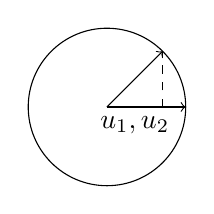
\begin{tikzpicture}
		\draw[->] (0,0) -- (1,0);
		\draw[->] (0,0) -- (0.707106781,0.707106781);
		\draw[thin] (0,0) circle (1);
		\draw[dashed] (0.707106781,0) -- (0.707106781,0.707106781);
		\draw[](0,0) -- node[below]{$\prs{u_1,u_2}$} (0.707106781,0); 
	\end{tikzpicture}
\end{center}
Le produit scalaire de deux vecteurs unitaires est donc le $\cos$ de l'angle $\theta$ entre les vecteurs.

De plus, on a la formule suivante : 
\[
	\prs{u,v} = \norm{u}\norm{v} \cos(\theta)
\]
et la propriété suivante (admise pour l'instant) 
\[
	\prs{u,v} \leq \norm{u}\norm{v}
\]

{\bf Interprétation en terme de projection ?}
{\bf formule du cos de l'angle en fonction des coordonnée?}

\subsubsection{Changement de base}

\begin{proposition}[(coordonnées d'un vecteur dans une bon)]
	Dans une base orthonormale $(e_1,e_2,e_3)$, un vecteur $u$ se décompose sous la forme\[
		x = \prs{e_1,x} e_1 + \prs{e_2,x} e_2 + \prs{e_3,x} e_3
	\]
\end{proposition}

\begin{proposition}[(Calcul du produit scalaire dans une bon)]
Si $(e_1,e_2,e_3)$ est une base orthonormée quelconque et si 
\[
	\begin{cases}
		u = u_1 e_1 + u_2 e_2 + u_3 e_3 \\
		v = v_1 e_1 + v_2 e_2 + v_3 e_3
	\end{cases}
\]
alors le produit scalaire $\prs{u,v} = u_1 v_1 + u_2v_2 + u_3v_3$.
\end{proposition}


\begin{definition}
	On définit la distance entre deux points $A$ et $B$ de l'espace par :
	\[
		d(A,B) = \norm{\overrightarrow{AB}}
	\]
	Si $\mathcal R$ est un repère orthonormé on a 
	\[
		d(A,B) = \sqrt{(x-x')^2+ (y-y')^2 + (z-z')^2 }
	\]
	où $\begin{psmallmatrix}
		x\\y\\z
	\end{psmallmatrix}_{\mathcal R}$ et $\begin{psmallmatrix}
		x'\\y'\\z'
	\end{psmallmatrix}_{\mathcal R}$ sont les coordonnées de $A$ et $B$ respectivement.
\end{definition}


\subsection{Produit mixte dans le plan}

\begin{definition}
[(Produit mixte)] 
Soit $u = (u_1,u_2)$  et $v = (v_1,v_2) $  deux vecteurs de $\R^2$. %Soit $(e_1,e_2)$ $\R^2$ muni d'une base orthonormée directe. 
On appelle \emph{déterminant} ou \emph{produit mixte} des deux vecteurs, le nombre réel
\[
	\det(u,v) =\begin{vmatrix}
			u_1 & v_1 \\
			u_2 & v_2
		\end{vmatrix} = u_1v_2 - u_2v_1. %\norm{u} \norm{v} \sin (\theta)
\]
%où 
%où $\theta$ est l'angle orienté entre les deux vecteurs.
\end{definition}

\begin{proposition}
	\begin{enumerate}
		\item Bilinéarité : soient trois vecteurs $u_1$ $u_2$ , $u_3$ et deux scalaires $(\lambda,\mu)\in \R$ :
			\begin{itemize}
				\item  $\det(\lambda u_1 + \mu u_2, u_3) = \lambda \det(u_1,u_3) + \mu \det(u_2,u_3) $
				\item $\det(u_1,\lambda u_2 + \mu u_3) = \lambda \det(u_1,u_2) + \mu \det(u_1,u_3)$ 
			\end{itemize}
		\item Antisymétrie : Pour tous $u,v\in\R^2$ on a $\det(u_1,u_2) = -\det(u_2,u_2)$.
	\end{enumerate}
\end{proposition}

\begin{remark}
	Attention donc à l'ordre d'écriture des facteurs dans le produit mixte!
\end{remark}

\begin{proposition}
	Soient $u,v$ deux vecteurs du plan. Les vecteurs $u$ et $v$ sont liés si et seulement si $\det(u,v) =0$.
\end{proposition}


\subsubsection{Interprétation  géométrique}

Le produit mixte de deux vecteurs $\det(u_1,u_2)$ représente l'aire algébrique du parallélogramme s'appuyant sur les deux vecteurs :
\begin{center}
	\includegraphics[height=5cm]{figures/produit_mixte.png}
\end{center}
%\begin{tikzpicture}[dot/.style={circle,inner sep=1pt,fill,label={#1},name=#1},
  %extended line/.style={shorten >=-#1,shorten <=-#1},
  %extended line/.default=1cm]
%\node [dot=A] at (0,0) {};
%\node [dot=B] at (2,1) {};
%\node [dot=P] at (1,3) {};

	%\draw[->,red,fill=red!50] (0,0) -- (2,1) --(3,4) -- (1,3) -- cycle ;

	%\draw[->,very thick] (0,0) -- (2,1);
	%\draw[->,very thick] (0,0) -- (1,3);

	%\draw [->] ($(A)!(P)!(B)$) -- (P);

%\end{tikzpicture}
De plus, si $\theta$ désigne l'angle orienté entre $u_1$ et $u_2$ on a 
\[
	\det(u_1,u_2) = \norm{u_1} \norm{u_2} \sin(\theta).
\]
En découle la propriété suivante :
\[
	\abs{\det(u,v)}\leq \norm{u} \norm{v}
\]
avec égalité si et seulement si les vecteurs sont orthogonaux.

\subsubsection{Changement de base}

\begin{proposition}[(Calcul du produit mixte dans une bon)]
Si $(e_1,e_2)$ est une base orthonormée quelconque et si 
\[
	\begin{cases}
		u = u_1 e_1 + u_2 e_2 \\
		v = v_1 e_1 + v_2 e_2 
	\end{cases}
\]
alors le produit mixte est $\det(u,v) =\begin{vmatrix}
			u_1 & v_1 \\
			u_2 & v_2
		\end{vmatrix}  = u_1 v_1 - u_2v_2$.
\end{proposition}

\subsection{Produit vectoriel dans l'espace}

\begin{proposition}
	Deux vecteurs $x =(x_1,x_2,x_3)$ et $y=(y_1,y_2,y_3)$ sont colinéaires si et seulement si
	\[
		\begin{vmatrix}
			x_1 & y_1 \\
			x_2 & y_2
		\end{vmatrix}= \begin{vmatrix}
			x_1 & y_1\\
			x_3 & y_3
		\end{vmatrix}=  \begin{vmatrix}
			x_2 & y_2\\
			x_3 & y_3
		\end{vmatrix} = 0
	\]
\end{proposition}

\begin{definition}
	On appelle \emph{produit vectoriel} de deux vecteurs $u=\begin{psmallmatrix}x_1,x_2,x_3\end{psmallmatrix} $ et $v=\begin{psmallmatrix}y_1,y_2,y_3\end{psmallmatrix} $ le vecteur :
	\[
		u \wedge v = \begin{pmatrix}
		\begin{vmatrix}
			x_2 & y_2\\
			x_3 & y_3
		\end{vmatrix}	,
		-\begin{vmatrix}
			x_1 & y_1\\
			x_3 & y_3
		\end{vmatrix},
			\begin{vmatrix}
			x_2 & y_2\\
			x_3 & y_3
		\end{vmatrix}
		\end{pmatrix}
	\]
\end{definition}

Le produit vectoriel $u\wedge v$ est orthogonal au plan engendré par $u$ et $v$ et sa norme est égale à l'aire du parallélogramme engendré par $u$ et $v$.
\begin{proposition}[(Propriété du produit vectoriel)]
	\begin{enumerate}
		\item	le produit vectoriel est bilinéaire :
			\begin{itemize}
				\item  $(\lambda u_1 + \mu u_2)\wedge u_3 = \lambda (u_1\wedge u_3) + \mu (u_2\wedge u_3) $
				\item $ u_1\wedge (\lambda u_2 + \mu u_3) = \lambda (u_1\wedge u_2) + \mu (u_1 \wedge u_3) $ 
			\end{itemize}

		\item	le produit vectoriel est antisymétrique : $u_1 \wedge u_2 = -u_1\wedge u_2$.
		\item Le produit vectoriel est nul si et seulement si les vecteurs sont colinéaires.
		\item	le produit vectoriel est un vecteur orthogonal aux deux vecteurs
			 $\prs{u_1, u_1 \wedge u_2} = \prs{u_2, u_1\wedge u_2 } =0 $
	\end{enumerate}
\end{proposition}

\subsubsection{Interprétation géométrique}
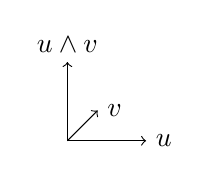
\begin{tikzpicture}
	\draw[->] (0,0,0) -- (1,0,0) node[right] {$u$};
	\draw[->] (0,0,0) -- (0,0,-1) node[right] {$v$};
	\draw[->] (0,0,0) -- (0,1,0) node[above] {$u\wedge v$};
\end{tikzpicture}

On a $\norm{u\wedge v} = sin(\theta)$.

\begin{definition}
	Soit $\mathcal B = (e_1,e_2,e_3)$ une base orthonormé. On dit que $\mathcal B$ est \emph{directe} si  $e_1 \wedge e_2 = e_3$. 
\end{definition}

\begin{remark}
	Dans une bon directe on a les égalités suivantes :
	\begin{itemize}
		\item	$ (e_1 \wedge e_2) \wedge e_3 = (e_3 \wedge e_1) \wedge e_2  = (e_1 \wedge e_3) \wedge e_2 = \cdots = 0$
		\item	$(e_1 \wedge e_2) \wedge e_1 = e_2 $,$(e_1 \wedge e_2) \wedge e_2 = -e_1 $, \ldots
	\end{itemize}

\end{remark}

\begin{proposition}
	[(Calcul du produit vectoriel dans une bon directe)]
Si $(e_1,e_2,e_3)$ est une base orthonormée directe, et si $u =x_1e_1+x_2e_2 + x_3e_3 $ et $v =y_1e_1+y_2e_2 + y_3e_3 $ alors
\[
		u \wedge v =
		\begin{vmatrix}
			x_2 & y_2\\
			x_3 & y_3
		\end{vmatrix} e_1 +
		-\begin{vmatrix}
			x_1 & y_1\\
			x_3 & y_3
		\end{vmatrix} e_2 + 
			\begin{vmatrix}
			x_2 & y_2\\
			x_3 & y_3
		\end{vmatrix} e_3
\]


\end{proposition}

\subsubsection{Double produit vectoriel}

Le produit vectoriel n'est pas associatif : 
En général, on a $(u\wedge v) \wedge w \neq u\weddge (v\wedge w)$. Plus précisément, on a la formule du double produit vectoriel
			
\begin{align*}
	u_1 \wedge (u_2 \wedge u_3) = \prs{u_1,u_3} u_2 - \prs{u_1,u_2} u_3
	(u_1 \wedge u_2) \wedge u_3 = \prs{u_1,u_3} u_2 -\prs{u_2,u_3} u_1
\end{align*}
En d'autre termes, $u_1 \wedge (u_2 \wedge u_3) $ appartient au plan engendré par $u_2$ et $u_3$ et $(u_1 \wedge u_2) \wedge u_3$ au plan $\vect(u_1,u_2)$


\subsection{Modes de repérage}

\subsubsection{Coordonnées polaires}

\subsubsection{Coordonnées cylindriques}

\subsubsection{Coordonnées sphériques}


\section{Représentation des fonctions de $\R^2$ et $\R^3$ à valeurs réelles}

\subsection{Rappels de bases}

\begin{definition}
	Soit $E$ et $F$ deux ensembles et  $f: E\to F$ une application de $E$ dans $F$ :
	\begin{itemize}
		\item Le domaine de définition de $f$ est l'ensemble $\D(f) \subset E$ des points de $E$ qui possèdent une image dans $F$ par $f$.
		\item L'image par $f$ de $\D$ est l'ensemble $Im(f) = \{ y\in F, \exists x\in E,  y = f(x)\} \subset F$.
		\item L'ensemble des points $\G(f) = \{(x, f(x))\in E \times F, x\in\D\}$ est appelé le graphe de $f$. %de $R n+1 est la surface représentative de f ; c’est l’analogue de la courbereprésentative d’une fonction d’une variable.
	\end{itemize}
\end{definition}

\begin{exemple}
La fonction $f:\R \to \R$ défini par $f(x) = \log(x(x+3)(x-2))$ a pour domaine de définition $\D(f) = ]-3,0[ \cup ]2,+\infty[$ :
	\begin{tikzpicture}
		\begin{axis}[axis x line=middle,axis y line=middle,ymin=-6,ymax=6,xmin=-4,xmax=6, after end axis/.code = {\draw[red!50,very thick] (axis cs:-3,0) -- (axis cs:0,0);\draw[red!50,very thick] (axis cs:2,0) -- (axis cs:6,0);}]
			\addplot[color=blue,id=excurve1,domain=-2.9999:-0.001,smooth,samples=800] gnuplot {log(x*(x+3)*(x-2))};
			\addplot[color=blue,id=excurve2,domain=2.0001:6,smooth,samples=800] gnuplot {log(x*(x+3)*(x-2))};
		\end{axis}
	\end{tikzpicture}
\end{exemple}

%\subsection{Représentation}
%\subsection{Ètude locale}
%\subsection{Étude globale}

\begin{definition}
		Une fonction $f$ de plusieurs variables à valeurs réelles (aussi appelé champs scalaire) est une fonction définie sur une partie $\D$ de $\R^n$ ($n\geq 1$) et à valeurs dans $\R$. Elle fait correspondre à tout point $\x =(x_1,x_2,\cdots,x_n)$ de $\D$ un unique point $y = f(\x)$ de $\R$.
\end{definition}

Dans la suite de ce chapitre nous donnerons principalement des exemples où $n=2$ et $n=3$. % et des champs de vecteurs (\ie le cas $n=m$). 

\begin{exemple} \label{exemple.fpv}
	\begin{itemize}
		\item	Le domaine de définition la fonction $f(x,y) = \sqrt{x+y}$ est l'ensemble $\D = \{(x,y) \in R^2, x + y \geq  0\}$. C'est la partie du plan suivante :
			\begin{center}
				\begin{minipage}{5cm}
					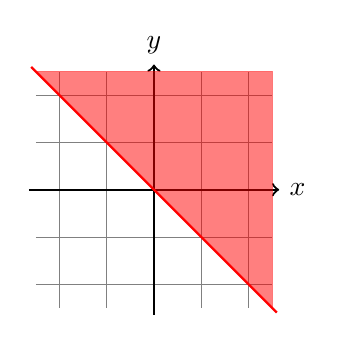
\begin{tikzpicture}[scale=.3]
	\def\xone{-5}
	\def\xtwo{5}
	\def\yone{-5}
	\def\ytwo{5}

% grid
  \draw[step=2cm,help lines] (\xone,\yone) grid (\xtwo,\ytwo);
  \draw[thick,->] (\xone-.3, 0) -- (\xtwo+.3, 0) node[right] {$x$};
  \draw[thick,->] (0, \yone-.3) -- (0, \ytwo+.3) node[above] {$y$};

% def domain
  \filldraw[red,opacity=.5] (\xone,\ytwo) -- (\xtwo,\ytwo) -- (\xtwo,\yone);
  \draw[red,thick] (\xone-.2,\ytwo+.2) -- (\xtwo+.2,\yone-.2);
  \node[] at (\xtwo/2,\ytwo/2) {$\D$};
\end{tikzpicture}
 
				\end{minipage}
				%\begin{minipage}{5cm}
					%%\begin{tikzpicture}
%	\begin{axis}[]
%	\addplot3[surf, shader=interp,samples=60, domain=-4:4, colormap/cool] {ln(x+y)};
%%	\addplot gnuplot [id=sin]{ sin(x) };
	%\addplot[mark=none, color=black]  plot gnuplot[samples=500,id=eins]{x**2/(1-x**2)};
% \end{axis}
%\end{tikzpicture}

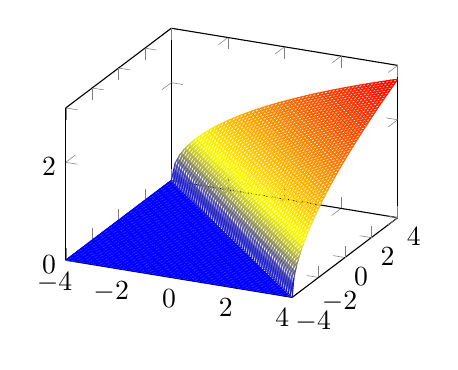
\begin{tikzpicture} 
%	\begin{axis}[
%			height=5cm,xlabel=$x$, ylabel=$y$, zlabel=$z$,zmin=0] 
%		\addplot3[surf,shader=flat,opacity=.8,samples=60] gnuplot {((x + y <0) && (x>3)) ?1/0}; 
%		%\addplot3[mesh,samples=60,domain=-4:4, y domain=-4:4]  {(sign(x+y)+1)/2*sqrt(abs(x+y))}; 
%		%\addplot3[white,surf,shader=interp,samples=50] {(x+y)sqrt(abs(x+y))}; 
%		%\filldraw[white] (axis cs:-4,-4,0) -- (axis cs:4,-4,0) -- (axis cs: -4,4,0); 
%\end{axis} 
	\begin{axis}[height=5cm,zmin=0]
		\addplot3[mesh,samples=60,domain=-4:4, y domain=-4:4]  {(sign(x+y)+1)/2*sqrt(abs(x+y))}; 
	\end{axis}
\end{tikzpicture}
	
				%\end{minipage}
			\end{center}
			Les valeurs prises par la fonction parcourent tout l'ensemble des réels positifs ou nuls : $Im(f) = \R^+$.
		\item Le domaine de définition de la fonction $f(x,y,z) = \ln(1 - |x| - |y| - |z|)$ est l'ensemble $\D = \big\{ (x,y,z)\in\R^3, |x|+|y|+|z| < 1 \big\}$ qui est représenté ci dessous :
			\begin{center}
				\begin{minipage}{5cm}
					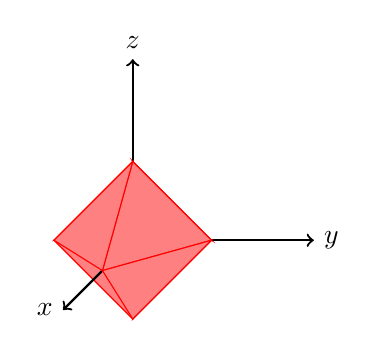
\begin{tikzpicture}
						\def\side{2}
						\draw[red,fill=red!50,opacity=1] (-1,0,0) -- (0,-1,0) -- (0,0,-1) --cycle ;
						\draw[red,fill=red!50,opacity=1] (1,0,0) -- (0,-1,0) -- (0,0,-1)--cycle ;
						\draw[red,fill=red!50,opacity=1] (-1,0,0) -- (0,1,0) -- (0,0,-1)--cycle ;
						\draw[red,fill=red!50,opacity=1] (1,0,0) -- (0,1,0) -- (0,0,-1)--cycle ;

						\draw[thick,->] (0,0,0) -- (\side+.3,0,0) node[right] {$y$};
						\draw[thick,->] (0,0,0) -- (0,\side+.3,0) node[above] {$z$};
						\draw[thick,->] (0,0,0) -- (0,0,\side+.3) node[left] {$x$};

						\draw[red,fill=red!50,opacity=1] (1,0,0) -- (0,1,0) -- (0,0,1) --cycle ;
						\draw[red,fill=red!50,opacity=1] (-1,0,0) -- (0,1,0) -- (0,0,1)--cycle ;
						\draw[red,fill=red!50,opacity=1] (1,0,0) -- (0,-1,0) -- (0,0,1)--cycle ;
					\end{tikzpicture}
				\end{minipage}
			\end{center}
	\end{itemize}
\end{exemple}


\subsection{Représentation du graphe}

Dans le cas des fonctions $f:\R^2 \to \R$, le graphe $\G(f) = \left\{ (x,y,f(x,y))\in \R^2 \times \R, (x,y) \in \D \right\}$ est un sous ensemble de $\R^3$. Lorsque la fonction $f:\R^2\to\R$ est régulière on peut représenter ce graphe comme une surface (on peut penser à un ``drap qui flotte'') dans $\R^3$. Lorsque $f$ est moins régulière, la représentation devient plus délicate et une étude locale de la fonction devient indispensable. 
Les axes $0x$ et $Oy$ (qui forme le plus souvent le plan horizontal) sont réservés aux variables $x$ et $y$ tandis que l'axe $Oz$ (le plus souvent l'axe vertical) représente la valeur de $z = f(x,y)$. Ainsi, pour tout $(x,y) \in \D(f)$ on a le point $(x,y,f(x,y)) \in \G(f)$. 
\begin{center}
	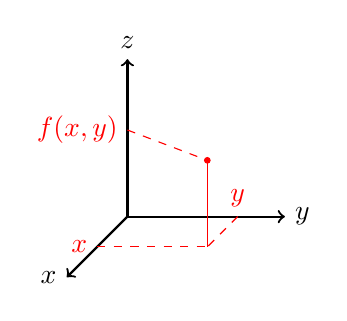
\begin{tikzpicture}

	\def\x{1}
	\def\y{1.4}
	\def\z{1.1}

	\def\siz{2}

	\draw[->,thick] (0,0,0) -- (0,0,\siz) node[left] {$x$} ;
	\draw[->,thick] (0,0,0) -- (\siz,0,0) node[right] {$y$} ;
	\draw[->,thick] (0,0,0) -- (0,\siz,0) node[above] {$z$} ;

	\draw[red] (\y,0,\x) -- (\y,\z,\x);
	\draw[red,dashed] (0,0,\x) node[left]{$x$} -- (\y,0,\x);
	\draw[red,dashed] (\y,0,0)  node[above]{$y$}-- (\y,0,\x);

	\node[above right] at (\y,\z,\x) {};

	%\draw[red,dashed] (0,0,\x) node[left]{$x$} -- (\y,\z,\x);
	\draw[red,dashed] (0,\z,0) node[left]{$f(x,y)$} -- (\y,\z,\x);
	\filldraw[red] (\y,\z,\x) circle (1pt);
	%\draw[red,dashed] (\y,0,0) node[left]{$x$} -- (\y,\z,\x);
\end{tikzpicture}

\end{center}

\begin{exemple}
	Voici quelques exemples de graphes de fonction de $\R^2$ dans $\R$. Les couleurs ne servent qu'à améliorer la lisibilité. 
	\begin{center}
		\begin{tabular}{cc}
			\begin{tikzpicture}
				\begin{axis}
					%\addplot3[surf,faceted color=blue, color=blue, domain=-4:4,samples=50,opacity=.3,fill opacity=.9,id=zaza] gnuplot {(x**3+y) * exp(-x**2-y**2)};
					\addplot3[surf,domain=-4:4,samples=50,colormap/cool,opacity=.8,id=zaza] gnuplot {(x**3+y) * exp(-x**2-y**2)};
				\end{axis}
			\end{tikzpicture}	&
			\begin{tikzpicture}
				\begin{axis}
					\addplot3[surf,domain=-10:10,samples=50,colormap/cool,opacity=.8,id=zozo]gnuplot {sin(sqrt(x**2 + y**2)) /sqrt(x**2 + y**2)};
				\end{axis}
			\end{tikzpicture}	                \\
			$f(x,y) = (x^3+y)\exp(-x^2-y^2)$&
			$f(x,y) = \sin(\sqrt{x^2 + y^2}) /\sqrt{x^2 + y^2}$\\
			\begin{tikzpicture}
				\begin{axis}
					\addplot3[surf,domain=-4:4,samples=50,colormap/cool,opacity=.8,id=zouzou] gnuplot {(x**2+y**2)};
				\end{axis}
			\end{tikzpicture}&
			\begin{tikzpicture}
				\begin{axis}
					\addplot3[surf,domain=-4:4,samples=50,colormap/cool,opacity=.8,id=zizi]gnuplot{(x**2-y**2)};
				\end{axis}
			\end{tikzpicture}\\
			Parabolloîde : $f(x,y) = x^2 + y^2$&
			Selle de cheval : $f(x,y) = x^2 - y^2$\\
		\end{tabular}
	\end{center}
\end{exemple}

\subsection{Représentation en couleur}

Une image en niveau de gris peut être modélisée par une fonction de deux variables à valeur réelle et définie sur le domaine $[0,1] \times [0,1]$.

\begin{exemple}
 Voici les fonctions du paragraphe précédent. Les couleurs code le signal comme l'indique la présence d'une échelle de couleurs à coté de chaque graphique. 
	\begin{center}
		\begin{tabular}{cc}
			\begin{tikzpicture}
			\begin{axis}[width=.45\textwidth,colorbar,colormap/cool,view={0}{90}]
					\addplot3[surf,domain=-4:4,samples=50,colormap/cool,opacity=.8,id=zaza] gnuplot {(x**3+y) * exp(-x**2-y**2)};
				\end{axis}
			\end{tikzpicture}	&
			\begin{tikzpicture}
				\begin{axis}[width=.45\textwidth,colorbar,colormap/cool,view={0}{90}]
					\addplot3[surf,domain=-10:10,samples=50,colormap/cool,opacity=.8,id=zozo]gnuplot {sin(sqrt(x**2 + y**2)) /sqrt(x**2 + y**2)};
				\end{axis}
			\end{tikzpicture}	                \\
			$f(x,y) = (x^3+y)\exp(-x^2-y^2)$&
			$f(x,y) = \sin(\sqrt{x^2 + y^2}) /\sqrt{x^2 + y^2}$\\
			\begin{tikzpicture}
				\begin{axis}[width=.45\textwidth,colorbar,colormap/cool,view={0}{90}]
					\addplot3[surf,domain=-4:4,samples=50,colormap/cool,opacity=.8,id=zouzou] gnuplot {(x**2+y**2)};
				\end{axis}
			\end{tikzpicture}&
			\begin{tikzpicture}
				\begin{axis}[width=.45\textwidth,colorbar,colormap/cool,view={0}{90}]
					\addplot3[surf,domain=-4:4,samples=50,colormap/cool,opacity=.8,id=zizi]gnuplot{(x**2-y**2)};
				\end{axis}
			\end{tikzpicture}\\
			Parabolloîde : $f(x,y) = x^2 + y^2$&
			Selle de cheval : $f(x,y) = x^2 - y^2$\\
		\end{tabular}
	\end{center}
\end{exemple}

\subsection{Représentation des ensembles de niveau}

\begin{definition}
	\'Etant donnée une fonction $\R^n \to \R$, l'\emph{ensemble de niveau} $\lambda \in Im(f)$ est $\left\{ \x\in\R^n, f(x) = \lambda \right\}$. 
\end{definition}
Dans le cas des fonctions de $\R^2$ dans $\R$, on parle de \emph{lignes de niveau}. On peut tracer les lignes de niveau en projettant sur le plan horizontal $z=0$ la courbe donnée par l'intersection du plan horizontal de hauteur $\lambda$ (\ie le plan d'équation $z=\lambda$) et le graphe de la fonction $f$. 
	\begin{center}
		\begin{tabular}{cc}
			\begin{tikzpicture}
				\begin{axis}[ domain=-2:2, domain y=0:2*pi, zmin = -1.8, ]

					\newcommand\expr[2]{exp(-#1^2) * sin(deg(#2))} %\newcommand\expr[2]{(.6*#2^2 + #1^2)}

					\addplot3[ contour gnuplot={ % cdata should not be affected by z filter:
							output point meta=rawz,
							number=10,
							labels=false,
						}, samples=41, z filter/.code=\def\pgfmathresult{-1.8}, ] {\expr{x}{y}};
					\addplot3[ contour gnuplot={
	    % cdata should not be affected by z filter:
							output point meta=rawz, number=10, labels=false, }, samples=41, ,thick ] {\expr{x}{y}};
					\addplot3[surf, samples=25,opacity=.01,fill opacity=.5]{\expr{x}{y}};
				\end{axis}
			\end{tikzpicture} &
			\begin{tikzpicture} 
				\newcommand\expr[2]{exp(-#1^2) * sin(deg(#2))}
				\begin{axis}[domain=-2:2,enlarge y limits, view={0}{90},  domain=-2:2,
						domain y=0:2*pi,
					] \addplot3[contour gnuplot={number=14},thick] {\expr{x}{y}}; \end{axis} \end{tikzpicture} \\
			représentation du graphe de $f(x,y) = \sin(y)e^{-x^2}$ & lignes de niveau de $f(x,y) = \sin(y)e^{-x^2}$
		\end{tabular}
	\end{center}

En pratique, on représente simultanément différentes courbes de niveau pour visualiser les différents niveau du graphe. Cette représentation s'apparente aux cartes géographiques où le niveau correspond à l'altitude. En bref, les courbes de niveau d'une fonction $f(x,y)$ fournissent une représentation géométrique de $f$ dans le plan, alors que son graphe en donne une dans l'espace.

\begin{exemple}
 Voici les lignes de niveau des fonctions du paragraphe précédent
	\begin{center}
		\begin{tabular}{cc}
			\begin{tikzpicture}
			\begin{axis}[width=.45\textwidth,colorbar,colormap/jet,view={0}{90}]
					\addplot3[samples=60,contour gnuplot={levels={0,0.0001,.001,.01,.1,.2,.3,.4,-.0001,-.001,-.01,-.1,-.2,-.3,-.4},labels=false
					},thick] gnuplot {(x**3+y) * exp(-x**2-y**2)};
				\end{axis}
			\end{tikzpicture}	&
			\begin{tikzpicture}
				\begin{axis}[width=.45\textwidth,colorbar,colormap/jet,view={0}{90}]
					\addplot3[samples=60,contour gnuplot={number=14,labels=false},thick]gnuplot {sin(sqrt(x**2 + y**2)) /sqrt(x**2 + y**2)};
				\end{axis}
			\end{tikzpicture}	                \\
			$f(x,y) = (x^3+y)\exp(-x^2-y^2)$&
			$f(x,y) = \sin(\sqrt{x^2 + y^2}) /\sqrt{x^2 + y^2}$\\
			\begin{tikzpicture}
				\begin{axis}[width=.45\textwidth,view={0}{90}]
					\addplot3[contour gnuplot={levels={0,1,2,3,4,5,6,7,8,9}},thick,contour/draw color={black}] gnuplot {(x**2+y**2)};
				\end{axis}
			\end{tikzpicture}&
			\begin{tikzpicture}
				\begin{axis}[width=.45\textwidth,view={0}{90}]
					\addplot3[contour gnuplot={number=14},thick,contour/draw color={black}]gnuplot{(x**2-y**2)};
				\end{axis}
			\end{tikzpicture}\\
			Parabolloîde : $f(x,y) = x^2 + y^2$&
			Selle de cheval : $f(x,y) = x^2 - y^2$\\
		\end{tabular}
	\end{center}
	Quelques exemples de la vie courante :
\begin{center}
	\begin{tabular}[]{cc}
		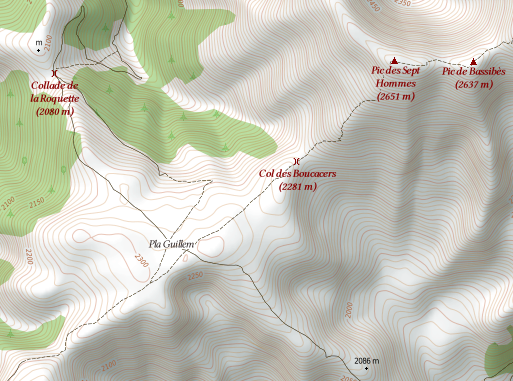
\includegraphics[height=4cm]{./figures/isohypses.png}
		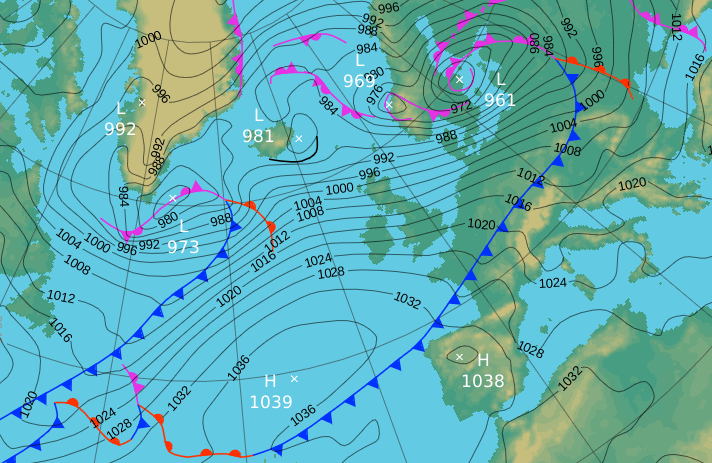
\includegraphics[height=4cm]{./figures/isobar.png}
	\end{tabular}
\end{center}
\end{exemple}

Pour les fonctions de $\R^3$ dans $\R$, les ensembles de niveau sont appelés \emph{surfaces de niveau}. Ces surfaces sont des sous ensembles de $\R^3$ et cela permet de représenter la fonction alors qu'il serait délicat de représenter son graphe qui est un sous ensemble de $\R^4$.  


\begin{exemple}
Lorsque la fonction $f:\R^3 \to \R$ est polynomial, on parle de surfaces algébriques. En voici deux exemples classiques :
	\begin{center}
		\begin{tabular}{p{.45\textwidth}c}
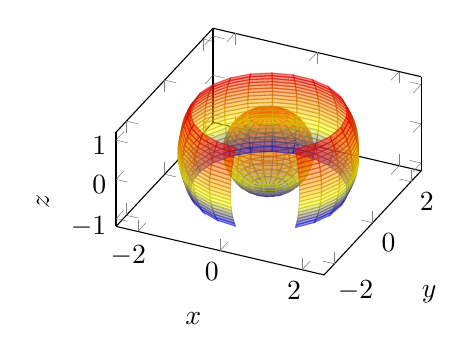
\begin{tikzpicture}
    \begin{axis}[%
	width=.45\textwidth,
        axis equal,
        %width=10cm,
        %height=10cm,
        %axis lines = center,
        xlabel = {$x$},
        ylabel = {$y$},
        zlabel = {$z$},
        %ticks=none,
        %enlargelimits=0.3,
        %view/h=45,
        %scale uniformly strategy=units only,
    ]
    \addplot3[ surf, opacity = 0.5, samples=21, domain=-1:1,y domain=0:2*pi, z buffer=sort] ({sqrt(1-x^2) * cos(deg(y))}, {sqrt( 1-x^2 ) * sin(deg(y))},
     x);
    \addplot3[ surf, opacity = 0.5, samples=21, domain=-1:1,y domain=-pi/4:2*pi-pi/2, z buffer=sort] ({sqrt(4-x^2) * cos(deg(y))}, {sqrt(4-x^2 ) * sin(deg(y))},
     x);
    \end{axis}

\end{tikzpicture}&
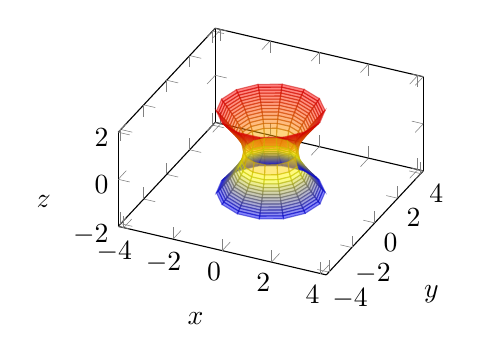
\begin{tikzpicture}
    \begin{axis}[width=.45\textwidth,
        axis equal,
            xmin=-2,xmax=2,
            ymin=-2,ymax=2,
            zmin=-2,zmax=2,
            xlabel={$x$},
            ylabel={$y$},
            zlabel={$z$},
            zlabel style={rotate=90},
            %view={60}{40}
    ]
        % x^2+y^2-z^2=1
        \addplot3[surf,opacity=.5,domain=1:2,y domain=0:2*pi,samples=15]({x*cos(deg(y))},{x*sin(deg(y))},{sqrt(x^2-1)});    
        \addplot3[surf,opacity=.5,domain=1:2,y domain=0:2*pi,samples=15]({x*cos(deg(y))},{x*sin(deg(y))},{-sqrt(x^2-1)});    

        % x^2+y^2-z^2=2
        %\addplot3[mesh,opacity=.5,domain=1:2,y domain=0:2*pi,samples=60,z buffer=sort]({x*cos(deg(y))},{x*sin(deg(y))},{(x*x-2)^.5 });    
        %\addplot3[mesh,opacity=.5,domain=1:2,y domain=0:2*pi,samples=60]({x*cos(deg(y))},{x*sin(deg(y))},{-(x*x-2)^.5 });    
    \end{axis}
\end{tikzpicture}\\												
			Sphere : surfaces de niveau $1$ et $4$ de la fonction $f(x,y) = x^2 + y^2 + z^2 $&
			Parabolloïde : la surface de niveau $1$ de  $f(x,y) = x^2 + y^2 - z^2 $
		\end{tabular}
	\end{center}


%	Bien d'autres exemple   \qrcode[hyperlink,height=1cm]{}
	Bien d'autres exemples  \fbox{ \qrcode[]{http://www.mathcurve.com/surfaces/algebricsu/algebricsu.shtml}}
\end{exemple}

\subsection{Les fonctions partielles}
%\'Etant donné une fonction $f:\R^n \to \R$, si on fixe la $i$-ème coordonné
\begin{definition}
	\'Etant donné une fonction $f:\R^n \to \R$, un nombre $a\in\R$ et un indice $i\in\left\{ 1,\cdots,n \right\}$ on note $\D_a^i(f) = \left\{ (x_1,\cdots,x_n) \in \R^n, x_i = a\right\} \cap \D(f)$. La fonction partielle $f^i_a:\R^{n-1} \to \R$ est définie par $f^i_a(y_1,\cdots,y_{n-1}) = f(y_1,\cdots,y_{i-1},a,y_{i},\cdots,y_{n-1})$ sur le domaine de définition  $\D(f^i_a) = \{ (y_1,\cdots,y_{n-1}) \in \R^{n-1}, (y_1,\cdots,y_{i-1},a,y_{i},\cdots,y_{n-1})\in \D(f) \}$.
\end{definition}

Dans le cas $n=2$ il y a deux fonctions partielles : si $f:\R^2 \to \R$ et $a\in\D(f)$ alors $f^1_a(\cdot) = f(a,\cdot)$ et $f^2_a (\cdot) = f(\cdot,a)$. Le graphe de ces deux fonction peut être déduit de l'intersection entre les plan (verticaux) d'équation $x=a$ et $y=a$ respectivement :

			\begin{tikzpicture}
				\def\cut{6}
				\def\formgnuplot{sin(sqrt(x**2 + y**2)) /sqrt(x**2 + y**2)};
				\def\form{sin(deg( (x^2 + (\cut) ^2)^.5)) /(x^2 + (\cut) ^2)^.5};
				\begin{axis}[xmin=-10,xmax=10,ymin=-10,ymax=10,zmin=-.3,zmax=1.3]
					\addplot3[surf,y domain=-10:10,domain=-10:\cut, samples=40,samples y= 50,colormap/cool,opacity=.8,id=zozo2]gnuplot {\formgnuplot};
					\draw[opacity=.5,fill=red!50,red] (axis cs: \cut,-10,-.3)-- (axis cs: \cut,10,-0.3) -- (axis cs: \cut,10,1.3) -- (axis cs: \cut,-10,1.3) -- cycle ;
					\addplot3[domain=-10:10,samples=50,samples y=0,red,ultra thick] (\cut,x,\form);
					\addplot3[surf,y domain=-10:10, domain = \cut:10,samples=10,samples y= 50,colormap/cool,opacity=.8,id=zozo]gnuplot {\formgnuplot};
				\end{axis}
			\end{tikzpicture}	                
			\begin{tikzpicture}
				\begin{axis}[xmin=-10,xmax=10,ymin=-.3,ymax=1.3]
				\def\cut{6};
			%	\def\formgnuplot{sin(sqrt(x**2 + y**2)) /sqrt(x**2 + y**2)};
				\def\form{sin(deg( (x^2 + (\cut) ^2)^.5)) /(x^2 + (\cut) ^2)^.5};
				\addplot[domain=-10:10,samples=60,blue,ultra thick] {\form};
				\end{axis}
			\end{tikzpicture}	                



			\begin{tikzpicture}
				\def\cut{-2};
				\begin{axis}[xmin=-10,xmax=10,ymin=-10,ymax=10,zmin=-.3,zmax=1.3]
					\addplot3[surf,domain=-10:10,y domain=\cut:10, samples=50,samples y= 30,colormap/cool,opacity=.8,id=zozo]gnuplot {sin(sqrt(x**2 + y**2)) / sqrt(x**2 + y**2)};
					\draw[opacity=.5,fill=red!50,red] (axis cs: -10,\cut,-.3)-- (axis cs: 10,\cut,-0.3) -- (axis cs: 10,\cut,1.3) -- (axis cs: -10,\cut,1.3) -- cycle ;
					\addplot3[domain=-10:10,samples=50,samples y=0,red,ultra thick] (x,\cut,{sin(deg( (x^2 + (\cut) ^2)^.5)) /(x^2 + (\cut)^2)^.5});
					\addplot3[surf,domain=-10:10, y domain = -10:\cut,samples=50,samples y= 20,colormap/cool,opacity=.8,id=zozo]gnuplot {sin(sqrt(x**2 + y**2)) / sqrt(x**2 + y**2)};
				\end{axis}
			\end{tikzpicture}	                
			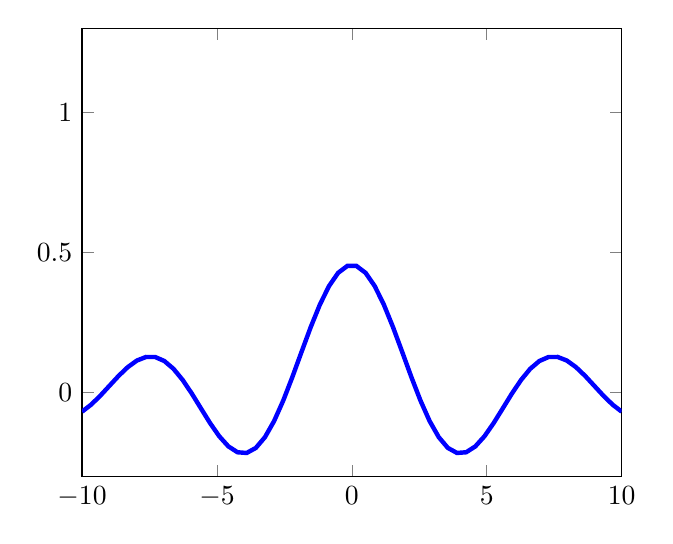
\begin{tikzpicture}
				\begin{axis}[xmin=-10,xmax=10,ymin=-.3,ymax=1.3]
				\def\cut{-2};
			%	\def\formgnuplot{sin(sqrt(x**2 + y**2)) /sqrt(x**2 + y**2)};
				\def\form{sin(deg( (x^2 + (\cut) ^2)^.5)) /(x^2 + (\cut) ^2)^.5};
				\addplot[domain=-10:10,samples=60,blue,ultra thick] {\form};
				\end{axis}
			\end{tikzpicture}	                

De même pour les fonctions de $\R^3\to \R$ on a


\section{Les fonction de plusieurs variables à valeurs vectoriel}

\subsection{Définition}

\begin{definition}
		 Une fonction $f$ de plusieurs variables à valeurs vectoriel (aussi appelé champs de vecteurs) est une fonction définie sur une partie $\D$ de $\R^n$ ($n\geq 1$) et à valeurs dans $\R^m$ ($m\geq 1$). Dans ce cas, il existe $p$ fonctions $f_1,\cdots,f_p$ . Elle fait correspondre à tout point $\x =(x_1,x_2,\cdots,x_n)$ de $\D$ un unique point $f(\x) = (f_1(\x),\cdots,f_m(\x)) =  (y_1,\cdots,y_m) = \y$ de $\R^m$.
\end{definition}

\subsection{Représentation des champs de vecteurs}

\begin{itemize}
	\item Le champs de vecteur $f(x,y) = \frac{0.15}{\sqrt{1+(x-y)^2}} \left(1, x-y\right )$ défini sur $\D = \R^2$ :
		\begin{center}
			\def\length{sqrt(1+(x-y)^2)}
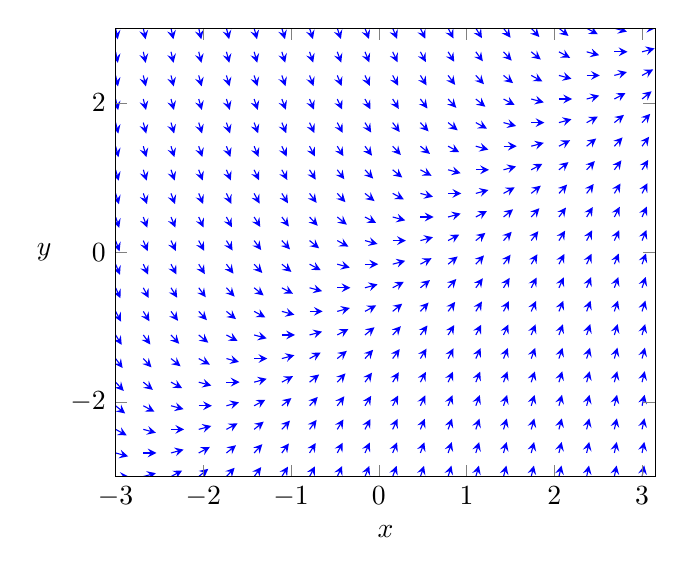
\begin{tikzpicture}
\begin{axis}[domain=-3:3, view={0}{90},xlabel = $x$,ylabel=$y$,ylabel style={rotate=-90},]
\addplot3[blue, quiver={u={1/(\length)}, v={(x-y)/(\length)}, scale arrows=0.15}, -stealth,samples=20] {0};
\end{axis}
\end{tikzpicture}

		\end{center}
	\item Un champs de vecteur $f:\R^3 \to \R^3$ défini sur $\D =\left\{ x^2 + y^2 + z^2 =1 \right\}$. On a $f(x,y,z) = (f(x,y,z),f_2(x,y,z),f_3(x,y,z)) \in \R^3$. En chaque point du domaine de définition on a donc un vecteur (``une flèche'') représenté par un champs de vecteur :
\end{itemize}
			\begin{center}
				%% helper macros
%: Styles for XYZ-Coordinate Systems
%: isometric  South West : X , South East : Y , North : Z
\tikzset{isometricXYZ/.style={x={(-0.866cm,-0.5cm)}, y={(0.866cm,-0.5cm)}, z={(0cm,1cm)}}}

%: isometric South West : Z , South East : X , North : Y
\tikzset{isometricZXY/.style={x={(0.866cm,-0.5cm)}, y={(0cm,1cm)}, z={(-0.866cm,-0.5cm)}}}

%: isometric South West : Y , South East : Z , North : X
\tikzset{isometricYZX/.style={x={(0cm,1cm)}, y={(-0.866cm,-0.5cm)}, z={(0.866cm,-0.5cm)}}}

%% document-wide tikz options and styles
\begin{tikzpicture} [scale=2, isometricZXY, line join=round,
        opacity=.75, text opacity=1.0,%
        %>=latex,
        inner sep=0pt,%
        outer sep=2pt,%
    ]
    \def\h{5}
    \shade[ball color=red!10!white,opacity=0.20] (0,0) circle (1.2cm);
    %Movement arrows
    \foreach \t in {225,235,...,295}
	\foreach \f in {50,40,...,0}
	    \draw [blue, opacity=1.0, ->, thick]
		({sin(\f - \h)*cos(\t - \h)}, {sin(\f - \h)*sin(\t - \h)}, {cos(\f - \h)})
		-- ({(1 + 0.2*cos(90 - \f))*sin(\f - \h)*cos(\t - \h)},
		    {(1 + 0.2*cos(90 - \f))*sin(\f - \h)*sin(\t - \h)},
		    {(1 + 0.2*cos(90 - \f))*cos(\f - \h)});

    \foreach \t in {125,135,...,205}
	\foreach \f in {110,100,...,0}
	    \draw [blue, <-, thick]
		({(1 + 0.2*cos(90 - \f))*sin(\f - \h)*cos(\t - \h)},
		 {(1 + 0.2*cos(90 - \f))*sin(\f - \h)*sin(\t - \h)},
		 {(1 + 0.2*cos(90 - \f))*cos(\f - \h)})
		-- ({sin(\f - \h)*cos(\t - \h)},{sin(\f - \h)*sin(\t - \h)},{cos(\f - \h)});
    \foreach \t in {35,45,...,115}
	\foreach \f in {130,120,...,0}
	    \draw [blue, opacity=1.0 ,->, thick]
		({sin(\f - \h)*cos(\t - \h)}, {sin(\f - \h)*sin(\t - \h)}, {cos(\f - \h)})
		-- ({(1 + 0.2*cos(90 - \f))*sin(\f - \h)*cos(\t - \h)},
		    {(1 + 0.2*cos(90 - \f))*sin(\f - \h)*sin(\t - \h)},
		    {(1 + 0.2*cos(90 - \f))*cos(\f - \h)});

    \foreach \t in {-55,-45,...,25}
	\foreach \f in {130,120,...,0}
	    \draw [blue, <-, thick]
		({(1 + 0.2*cos(90 - \f))*sin(\f - \h)*cos(\t - \h)},
		 {(1 + 0.2*cos(90 - \f))*sin(\f - \h)*sin(\t - \h)},
		 {(1 + 0.2*cos(90 - \f))*cos(\f - \h)})
	      -- ({sin(\f - \h)*cos(\t - \h)},{sin(\f - \h)*sin(\t - \h)},{cos(\f - \h)});

\end{tikzpicture}

			\end{center}

\section{Les courbes du plan et de l'espace}

